SyVOLT is a user-friendly Eclipse plugin to verify pre-/post- condition
contracts on model transformations specified in the DSLTrans transformation
language. The tool has a number of unique features, outlined below.

\subsection{Integration with Eclipse}

Eclipse is a popular development environment and model transformation
tools such as ATL [CITE], DSLTrans [CITE] and EGL [CITE] are integrated with the
Eclipse Modeling Framework (EMF) [CITE].
To take advantage of this ecosystem, SyVolt also integrates with EMF.

In the EMF, models can be represented in a multitude of syntaxes, from graphical
to textual, and this makes the interaction with SyVolt easier since the modeler
can use the model editor that is most convenient. Internally, SyVolt uses 
the Himesis format [CITE] to represent models.

\subsection{Model Driven Developed GUI}

To take advantage of the productivity promised by MDD, we used a language called
Eugenia[CITE] to generate the SyVolt contract editor shown in
Figure~\ref{fig:eclipse_frontend}.

Eugenia consists of a set of annotations that are attached to the metamodel of
SyVolt contracts and, without any extra information, generates a set of eclipse
Graphical Modeling Framework (GMF) models.
Each GMF model is concerned with one aspect of the editor and can be further
customized to our needs.
For instance, the generated GMF tooling model prescribes the kind of tools that
will be available in the toolbox (shown in the right of
Figure~\ref{fig:eclipse_frontend}), their icons, labels, etc\ldots From the set
of GMF models, a set of eclipse plugins are synthetize that, when installed,
make up the graphical editor\footnote{A fixed structure textual editor is also provided but this editor lacks several usability improvements and, hence, is not appropriate to model SyVolt contracts.}.

\begin{figure}
\centering
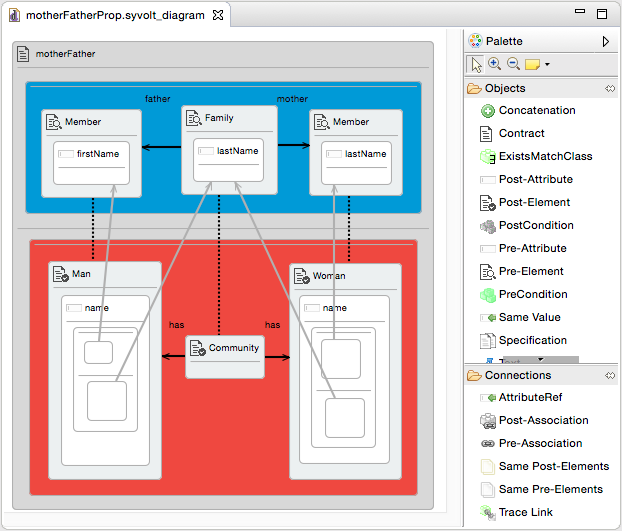
\includegraphics[width=0.45\textwidth]{figures/eclipse_frontend}
\caption{The transformation editor within Eclipse}
\label{fig:eclipse_frontend}
\end{figure}

With this approach, SyVolt editor was developed in about 4 man-hours.

\subsection{Graphical Modelling}

Due to the graph-like structure of the pre and post conditions of contracts, the
visual representation of the contract in SyVolt editor allows the user to
quickly build and intuitively understand their meaning.
If a textual (logical or mathematical) editor where to be used, the user would
need an extra system of identifiers to correctly prescribe the structure of contracts.

The visual representation of a contract has all the necessary information to derive the correct 
logical expression to be used by the internal SyVolt prover.

\subsection{Import from ATL}
The Atlas Transformation Language (ATL) is commonly-used in both industry and
academia applications. In order to extend our approach into these domains, we
have developed a higher-order transformation that is able to automatically
transform declarative ATL transformations into our transformation language
DSLTrans~\cite{Oakes}. This allows the user to exhaustively prove contracts on
ATL transformations.

\subsection{Symbolic Execution}
We apply the symbolic execution technique clasically used for program
verification, to the verification of model transformations. The DSLTrans
transformations and contracts are built upon typed graphs.
Our contract prover is able to reason over these graphs to prove contracts. An
example of this would be in the Families-To-Persons transformation from the ATL
zoo [CITE]. In this transformation, the name for a person in the output graph is
a concatenation of two strings from elements in the input graph. Our contract
prover can prove that this concatenation will be valid in all cases.

\subsection{Push-Button Proving}
Hidden formal methods: providing the transformation and the contract is
sufficient for the tool to automatically provide formal guarantees of correctness. Once the transformation
and the contracts of interest are created, one command will start the property proving process. This process will automatically create
all required artifacts (as detailed in the following section), run the process,
and then provide the results to the user within the Eclipse environment, as seen
in Figure~\ref{fig:output}. This allows the user to continually stay within the
Eclipse environment.

\begin{figure}
\centering
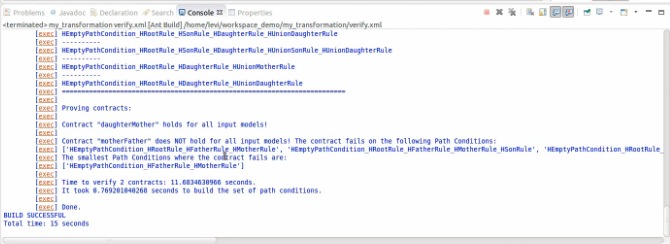
\includegraphics[width=0.45\textwidth]{figures/output}
\caption{The results of the contract prover}
\label{fig:output}
\end{figure}

\subsection{Input Independence and Exhaustiveness}

Our technique will exhaustively prove whether a contract will hold for all
possible input models to a transformation. This allows us to exhaustively verify
a transformation, as seen in~\cite{Lucio2014}.

\subsection{Proving Speed}

SyVOLT scales to transformations of practical interest. This has been probed
empirically by applying it to DSLTrans transformations up to X rules, and ATL
transformations up to Y rules. The average size of a DSLTrans transformation is
around XX rules (cite something here) and of ATL rules around YY rules. Even
though our technique is exhaustive, our approach takes a relatively short amount
of time to prove contracts. For example, our experiments on industrial
transformations~\cite{Oakes} show that contracts can be verified within a few
minutes. \cite{Selim2014} demonstrates that our prover is faster than similar
approaches based on SAT solvers.

\subsection{Production of Counter-Examples}

An advantage of our technique is that a counter-example model for a particular
contract can be produced by the contract proving process. This allows the user
to easily determine the error in the transformation and correct it. We suggest
that this enables a transformation development method analogous to 'test-driven
development'. In this method, development would be routinely punctuated by
contract proof in order to catch errors early.

 